\documentclass[11pt]{article}
\usepackage[margin=1in]{geometry}
\usepackage{amsmath,amssymb}
\usepackage{graphicx}
\usepackage{tikz}
\usetikzlibrary{calc}
\usepackage{pgfplots}
\pgfplotsset{compat=1.17}

\title{Comprehensive Review: Generalization in Boosting}
\author{Master's Level Data Science}
\date{}

\begin{document}
\maketitle
\tableofcontents
\bigskip

\section{Introduction}
This review synthesizes the lecture slides (\texttt{ensemble-3.pdf}) and audio transcript (\texttt{GeneralizationBoosting.txt}) on the surprising generalization behavior of AdaBoost. We cover:
\begin{itemize}
  \item Recap of AdaBoost and its training error bound.
  \item Empirical observations on overfitting.
  \item The notion of \emph{margin} and its role in generalization.
  \item Exponential loss interpretation and coordinate‐descent view.
  \item Practical insights and extensions.
\end{itemize}

\section{AdaBoost Recap and Training Error Bound}
Given data $\{(x_i,y_i)\}_{i=1}^n$, $y_i\in\{-1,+1\}$, AdaBoost initializes weights
\[
  D_1(i)=\frac1n,
\]
and for $t=1,\dots,T$:
\begin{enumerate}
  \item Train weak learner on $D_t$ to obtain $h_t:X\to\{-1,+1\}$.
  \item Compute weighted error
  \[
    \varepsilon_t \;=\;\sum_{i=1}^n D_t(i)\,\mathbf{1}[h_t(x_i)\neq y_i].
  \]
  \item Set classifier weight
  \[
    \alpha_t \;=\;\tfrac12\ln\!\Bigl(\frac{1-\varepsilon_t}{\varepsilon_t}\Bigr).
  \]
  \item Update and normalize:
  \[
    D_{t+1}(i)\propto D_t(i)\,\exp\bigl(-\alpha_t\,y_i\,h_t(x_i)\bigr).
  \]
\end{enumerate}
The final classifier is
\[
  H(x)=sign\Bigl(\sum_{t=1}^T \alpha_t\,h_t(x)\Bigr).
\]
If each weak learner has edge $\gamma_t=\tfrac12-\varepsilon_t>0$, then the training error satisfies
\[
  \frac1n\sum_{i=1}^n\mathbf{1}[H(x_i)\neq y_i]
  \;\le\;\exp\!\Bigl(-2\sum_{t=1}^T\gamma_t^2\Bigr)
  \;\le\;\exp\!\bigl(-2T\gamma^2\bigr),
\]
where $\gamma=\min_t\gamma_t$. Thus training error decays \emph{exponentially} in $T$.

\section{Empirical Observations on Overfitting}
Experiments on the UCI ``letter'' dataset by Freund and Schapire showed:
\begin{center}
\begin{tabular}{r|ccc}
\hline
\# Rounds & 5 & 100 & 1000 \\
\hline
Train error (\%) & 0.0 & 0.0 & 0.0 \\
Test error (\%)  & 8.4 & 3.3 & 3.1 \\
\hline
\end{tabular}
\end{center}
Despite growing to over two million nodes (1000 trees), test error \emph{kept decreasing}, contradicting the usual overfitting expectation.

\section{Margins and Generalization}
Define the \emph{normalized score}
\[
  f(x)\;=\;\frac{\sum_{t=1}^T\alpha_t\,h_t(x)}{\sum_{t=1}^T\alpha_t},
\]
and the \emph{margin} on $(x_i,y_i)$ by
\[
  \text{margin}_i \;=\; y_i\,f(x_i)\;\in\;[-1,1].
\]
A positive margin implies correct classification; larger margins reflect stronger confidence. Empirically:
\begin{itemize}
  \item At 5 rounds: minimum margin $\approx0.14$.
  \item At 100 rounds: minimum margin $\approx0.52$.
  \item At 1000 rounds: minimum margin $\approx0.55$.
\end{itemize}
Even after zero training error, AdaBoost \emph{continues to increase margins}, which correlates with improved test performance.

\section{Exponential Loss and Coordinate Descent View}
Boosting can be viewed as minimizing the \emph{exponential loss}
\[
  L(f)\;=\;\frac1n\sum_{i=1}^n e^{-y_i f(x_i)},
\]
an upper bound on the 0-1 loss. In the (potentially infinite) feature mapping
\[
  \phi(x) = \bigl(h(x)\bigr)_{h\in\mathcal H},
\]
AdaBoost learns a linear classifier $f(x)=w\cdot\phi(x)$ by \emph{coordinate descent}, each round adjusting one coordinate (the new weak classifier) to descend the exponential loss.

\section{Geometric Illustration}
\begin{figure}[h]
\centering
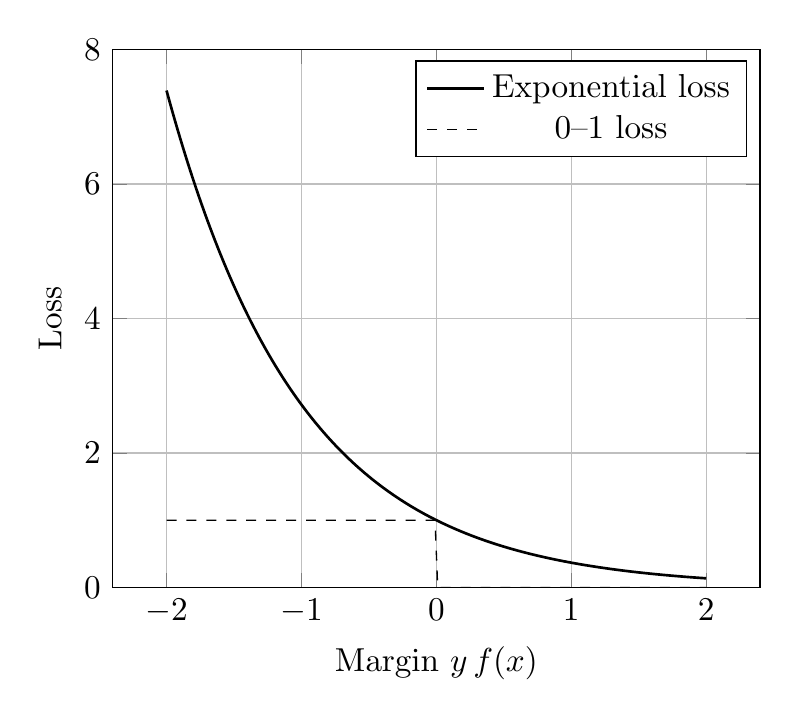
\begin{tikzpicture}[scale=1.2]
  \begin{axis}[
    xlabel={Margin $y\,f(x)$},
    ylabel={Loss},
    domain=-2:2, samples=200,
    ymin=0, ymax=8,
    grid=both
  ]
    \addplot[thick] {exp(-x)};
    \addlegendentry{Exponential loss}
    \addplot[dashed] {x<0 ? 1 : 0};
    \addlegendentry{0--1 loss}
  \end{axis}
\end{tikzpicture}
\caption{Exponential loss (solid) vs.\ 0--1 loss (dashed) as a function of margin.}
\end{figure}

\section{Algorithm Summary}
\begin{enumerate}
  \item Initialize uniform weights $D_1(i)=1/n$.
  \item For $t=1,\dots,T$:
    \begin{enumerate}
      \item Train weak learner under $D_t$ to get $h_t$.
      \item Compute $\varepsilon_t$, set $\alpha_t=\tfrac12\ln((1-\varepsilon_t)/\varepsilon_t)$.
      \item Update and renormalize $D_{t+1}(i)\propto D_t(i)\exp(-\alpha_t y_i h_t(x_i))$.
    \end{enumerate}
  \item Output $H(x)=sign(\sum_t\alpha_t h_t(x))$.
\end{enumerate}

\section{Interpretation \& Guidelines}
\begin{itemize}
  \item \textbf{Margin maximization} drives generalization even after zero training error.
  \item \textbf{No overfitting} often observed: boosting focuses on increasing margins rather than merely fitting labels.
  \item \textbf{Monitoring}: one may stop when margin gains plateau rather than when training error hits zero.
  \item \textbf{Extensions}: adding shrinkage or early stopping can further control complexity.
\end{itemize}

\section{Future Directions / Extensions}
\begin{itemize}
  \item \textbf{Gradient Boosting}: adapt boosting to arbitrary differentiable losses.
  \item \textbf{Regularized Boosting}: incorporate shrinkage (learning rate), subsampling (stochastic GBM).
  \item \textbf{Multi-class Boosting}: SAMME, multinomial boosting approaches.
  \item \textbf{Kernelized Boosting}: combine boosting with kernel methods for richer feature mappings.
\end{itemize}

\end{document}
